\documentclass{standalone}
\usepackage{pgfplots}

\begin{document}
    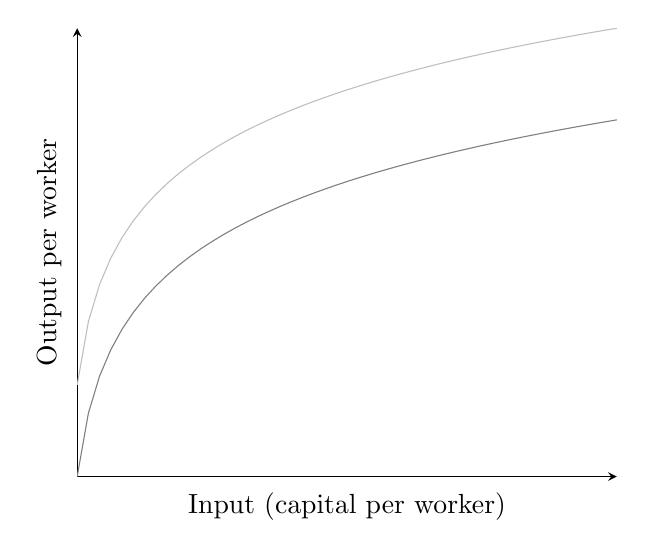
\begin{tikzpicture}
        \begin{axis}[
            axis lines = left,
            xlabel = {Input (capital per worker)},
            ylabel = {Output per worker},
            ytick=\empty,
            xtick=\empty,
            ]
            \addplot [domain=0:4,samples=50, gray] {ln(x)} node[right] {$y=G(N)f(k)$};
            \addplot [domain=0:4,samples=50, gray!50] {ln(x)+1} node[right] {$y=G(N')f(k)$};
        \end{axis}
    \end{tikzpicture}
\end{document}